\documentclass[twocolumn]{article}
\usepackage[utf8]{inputenc}
\usepackage{graphicx}
\usepackage{amsmath,amssymb}
\usepackage{booktabs}
\usepackage{caption}
\usepackage{subcaption}
\usepackage{geometry}
\geometry{margin=1in}

\title{The Incumbent Tax: A Stochastic Assessment of Pre-Election Clientelism and Fiscal Insolvency in Philippine LGUs}
\author{ICARE 2025 Policy Hackathon Team}
\date{}

\begin{document}

\maketitle

\begin{abstract}
Political budget cycles (PBCs) are a well-documented phenomenon in developing democracies, yet the fiscal risk implications of pre-election patronage remain underexplored. We combine 31 years of Philippine local government unit (LGU) panel data (1992--2022) with a forward-looking Monte Carlo simulation (10,000 iterations) to quantify the electoral returns and fiscal costs of opportunistic spending. Our empirical voter elasticity model---estimated via LGU fixed effects---suggests that public welfare spending has minimal electoral impact ($\hat{\beta}=0.00026$, $p=0.150$), while education and health expenditures yield slightly higher but still modest returns ($\hat{\beta}=0.00276$, $p=0.007$; $\hat{\beta}=0.00136$, $p=0.136$). We simulate two scenarios: a clientelistic surge (+24.3\% spending) and a normative balanced human-capital portfolio. The clientelistic surge produces a marginal (and statistically insignificant) vote-share decline ($-0.0011$), while increasing the expected deficit by PHP 37.64M, elevating 95\% Value-at-Risk by PHP 38.64M, and raising the probability of 10-year cumulative insolvency from 54.9\% to 73.8\%. These results are consistent with the hypothesis that pre-election patronage constitutes an ``incumbent tax'': incumbents appear to pay a substantial fiscal price with little observable electoral reward. Our findings directly inform SDG 16 (inclusive institutions) and SDG 1/3/4 (poverty, health, education) by highlighting how misallocated spending can undermine fiscal sustainability and service delivery. We propose dynamic fiscal guardrails and pre-election spending ceilings as immediate policy interventions.
\end{abstract}

\section{Introduction}

Political budget cycles (PBCs)---the systematic manipulation of fiscal policy in election years---are pervasive in developing countries \cite{akhmedov2004opportunistic, drazen2006electoral}. Incumbents often increase public spending before elections to signal competence or to buy votes \cite{keefer2005electoral, golden2014distributive}. In the Philippines, local chief executives have been shown to inflate expenditures on public works and welfare programs ahead of elections \cite{capuno2016patronage, llanto2016local}. However, the literature has largely focused on static econometric regressions that treat budgets as deterministic outcomes, with less attention to the stochastic nature of revenues and the tail-risk exposure generated by pre-election overspending. Subnational fiscal risk frameworks (e.g., World Bank and IMF subnational debt sustainability assessments; see also \cite{glasserman2003monte} for related simulation methodology) have been developed elsewhere, but to our knowledge, no study has combined a panel elasticity model with a Monte Carlo simulation to assess the electoral–fiscal trade-off for Philippine LGUs.

This paper addresses this gap by introducing a forward-looking stochastic simulation framework that quantifies the trade-off between electoral survival and fiscal sustainability. We ask: (1) Does pre-election budget expansion yield meaningful electoral gains? (2) What is the estimated fiscal cost of clientelistic spending in terms of deficits, insolvency risk, and tail-risk exposure? (3) Does patronage reduce political uncertainty for the incumbent?

Our approach proceeds in three steps. First, we estimate voter elasticities from a panel of Philippine LGUs (1992--2022) using LGU fixed effects, controlling for time-invariant heterogeneity. Second, we model the joint distribution of local revenue sources (taxes and IRA) using a lognormal distribution with Cholesky-induced correlation, and simulate 10,000 revenue--expenditure paths. Third, we compare two counterfactual scenarios: a clientelistic surge (Scenario A) that mirrors pre-election spending patterns, and a normative balanced human-capital portfolio (Scenario B) that reallocates funds toward education and health as a counterfactual policy.

The results suggest that the clientelistic surge, despite increasing total spending by PHP 37.64M (24.3\%), produces a marginal and non-positive electoral effect: mean vote share decreases from 50.89\% to 50.78\%. Meanwhile, it reverses a small surplus (PHP 3.34M) into a deficit (PHP 34.30M), raises the 95\% Value-at-Risk deficit by PHP 38.64M, and drives the probability of 10-year cumulative insolvency from 54.9\% to 73.8\%. We interpret this pattern as an ``incumbent tax''---a fiscal burden that incumbents appear to impose on their own jurisdiction without clear electoral compensation. These findings are directly relevant to SDG 16 (peace, justice, and strong institutions) and SDG 1, 3, and 4 (poverty reduction, health, and education), as they highlight governance failures that can undermine service delivery and fiscal resilience.

The remainder of the paper is structured as follows. Section 2 details the data and methodology. Section 3 presents the results. Section 4 discusses the implications and limitations. Section 5 concludes with policy recommendations.

\section{Methodology}

\subsection{Data}

We use a 31-year panel (1992--2022) of Philippine cities and municipalities, merging fiscal data from the Bureau of Local Government Finance (BLGF) with electoral data from the Commission on Elections (COMELEC). The dataset includes 227 provinces, cities, and municipalities, with annual observations on:

\begin{itemize}
\item \textbf{Fiscal variables:} total locally sourced revenue (\texttt{totlocsrc}), Internal Revenue Allotment (IRA), expenditures by sector (public welfare, general administration, education, health), and total expenditure.
\item \textbf{Electoral variables:} incumbent vote share ($\pi$), effective number of candidates (ENC\_lt), and pre-election year indicators.
\end{itemize}

The data were cleaned by removing non-numeric characters, converting zeros in sectoral expenditures to missing (following the codebook's advice), and winsorizing the top 1\% of fiscal variables to reduce outlier influence. The final estimation sample includes 1,847 LGU-year observations with complete data for the voter elasticity model. The panel is unbalanced, with an average of approximately 8 observations per LGU over the 31-year period; within-unit variation is sufficient for fixed effects identification, though attrition should be noted.

Table~\ref{tab:summary} reports summary statistics for the main variables.

\begin{table}[ht]
\centering
\caption{Summary Statistics (Full Sample)}
\label{tab:summary}
\small
\begin{tabular}{lrrrr}
\toprule
Variable & Mean & Std. Dev. & Min & Max \\
\midrule
Tot. local revenue (PHP M) & 149.2 & 34.8 & 5.2 & 310.1 \\
IRA (PHP M) & 448.5 & 39.7 & 120.3 & 520.4 \\
Vote share ($\pi$) & 0.651 & 0.194 & 0.012 & 0.999 \\
ENC\_lt & 2.48 & 1.12 & 1.00 & 7.23 \\
Public welfare exp. (PHP M) & 52.3 & 18.7 & 0 & 98.4 \\
Education exp. (PHP M) & 28.6 & 12.4 & 0 & 55.2 \\
Health exp. (PHP M) & 24.1 & 10.8 & 0 & 48.9 \\
\bottomrule
\end{tabular}
\end{table}

\subsection{Empirical Voter Elasticity Model}

We estimate the following fixed-effects model using LGU-level demeaned data:

\begin{equation}
\begin{aligned}
\pi_{it} - \bar{\pi}_i = &\ \beta_1 \left(\ln(\text{pubwelf}_{it}+1) - \overline{\ln(\text{pubwelf}+1)}_i\right) \\
&+ \beta_2 \left(\ln(\text{educexp}_{it}+1) - \overline{\ln(\text{educexp}+1)}_i\right) \\
&+ \beta_3 \left(\ln(\text{healthexp}_{it}+1) - \overline{\ln(\text{healthexp}+1)}_i\right) \\
&+ \beta_4 \left(\text{ENC}_{it} - \overline{\text{ENC}}_i\right) + \varepsilon_{it}.
\end{aligned}
\end{equation}

This specification removes LGU-specific time-invariant characteristics (e.g., political culture, geography) that could confound the relationship between spending and votes. The coefficients are estimated by OLS on the demeaned data. Results are reported in Table~\ref{tab:elasticities}.

\begin{table}[ht]
\centering
\caption{Fixed-Effects Voter Elasticities}
\label{tab:elasticities}
\small
\begin{tabular}{lcccc}
\toprule
Variable & Coefficient & Std. Error & $t$-stat & $p$-value \\
\midrule
$\ln(\text{pubwelf}+1)$ & 0.00026 & 0.00018 & 1.44 & 0.150 \\
$\ln(\text{educexp}+1)$ & 0.00276 & 0.00102 & 2.71 & 0.007 \\
$\ln(\text{healthexp}+1)$ & 0.00136 & 0.00091 & 1.49 & 0.136 \\
ENC\_lt & -0.2697 & 0.0923 & -2.92 & 0.004 \\
\bottomrule
\end{tabular}
\par\smallskip
\footnotesize{Adjusted $R^2 = 0.21$, $N = 1,847$. The adjusted intercept is computed as $\bar{\pi} - \hat{\beta}_1\overline{\ln(\text{pubwelf}+1)} - \hat{\beta}_2\overline{\ln(\text{educexp}+1)} - \hat{\beta}_3\overline{\ln(\text{healthexp}+1)} - \hat{\beta}_4\overline{\text{ENC}}$, ensuring that predictions at mean predictors equal the overall mean vote share.}
\end{table}

The small coefficients on expenditures suggest that marginal changes in sectoral spending have limited electoral payoffs, while a higher effective number of candidates is associated with a significantly lower vote share. The coefficient on education is statistically significant at the 1\% level, while public welfare and health are not individually significant; however, the combined human-capital effect (education + health) is additively larger than public welfare alone. The model explains about 21\% of the within-LGU variation in vote share, indicating that while the identified relationships are informative, much of the electoral outcome remains determined by unobserved factors.

\subsection{Monte Carlo Simulation Framework}

\subsubsection{Revenue Processes}
We model local revenue ($\text{Loc}_t$) and IRA ($\text{IRA}_t$) as jointly lognormal:

\[
\begin{pmatrix}
\ln \text{Loc}_t \\
\ln \text{IRA}_t
\end{pmatrix} \sim \mathcal{N}\left( \boldsymbol{\mu}, \boldsymbol{\Sigma} \right),
\]

where $\boldsymbol{\mu}$ is derived from the sample means and variances using the method of moments, and $\boldsymbol{\Sigma}$ includes the empirical correlation ($\rho=0.45$) between the two sources. We generate 10,000 draws via Cholesky decomposition. Total income $Y_t = \text{Loc}_t + \text{IRA}_t$.

\subsubsection{Expenditure Scenarios}
We construct two counterfactual spending policies:

\begin{enumerate}
\item \textbf{Scenario A (Clientelistic Surge):} Total expenditure = $(1 + s_t) \times \bar{Y}$, where $s_t \sim \mathcal{U}(0.15,0.30)$. The allocation shares (35\% public welfare, 35\% general administration, 15\% education, 15\% health) reflect the average pre-election expenditure composition observed in Figure~\ref{fig:pbc}. These shares were derived by computing the mean sectoral shares across all pre-election years in the data; the pattern shows that public welfare and general administration dominate the spending surge.

\item \textbf{Scenario B (Normative Human-Capital Portfolio):} Total expenditure = $(1 + s_t) \times \bar{Y}$, with $s_t \sim \mathcal{U}(-0.05,0.02)$. The allocation shares (10\% public welfare, 25\% general administration, 35\% education, 30\% health) are a \emph{counterfactual} reallocation toward education and health, designed to illustrate the fiscal and electoral consequences of redirecting funds from patronage to human-capital investments.
\end{enumerate}

We then compute the deficit $D_t = \text{Exp}_t - Y_t$ and define insolvency as $D_t / Y_t > 0.05$.

\subsubsection{Voter Response}
Vote share $\pi_t$ is simulated using the estimated elasticities and residual noise:

\begin{equation}
\begin{aligned}
\pi_t = &\ \hat{\alpha} + \hat{\beta}_1 \ln(\text{pubwelf}_t+1) \\
&+ \hat{\beta}_2 \ln(\text{educexp}_t+1) \\
&+ \hat{\beta}_3 \ln(\text{healthexp}_t+1) \\
&+ \hat{\beta}_4 \text{ENC}_t + \varepsilon_t,
\end{aligned}
\end{equation}

where $\varepsilon_t \sim \mathcal{N}(0, \hat{\sigma}^2)$ and $\hat{\sigma}=0.0652$. This allows us to calculate the mean vote share and its volatility across simulations.

\subsubsection{Cumulative Deficit Tracker}
We also simulate a 10-year horizon (reflecting electoral cycles) where income and expenditures follow the same distributions (with persistence in the surge multiplier). Cumulative insolvency is flagged if $\sum_{t=1}^{10} D_t / \sum_{t=1}^{10} Y_t > 0.05$.

All simulations were conducted in Python 3.10 using NumPy 1.24 and pandas 2.0 with a fixed random seed (42) for reproducibility.

\section{Results}

\subsection{Empirical Political Budget Cycle}
Figure~\ref{fig:pbc} displays the mean sectoral expenditures in pre-election vs. off-election years. Public welfare and general administration expenditures are higher in pre-election years, consistent with the presence of a PBC in Philippine LGUs. Specifically, public welfare spending increases by 18.4\% and general administration by 12.7\% in election years relative to off-election years.

\begin{figure}[ht]
\centering
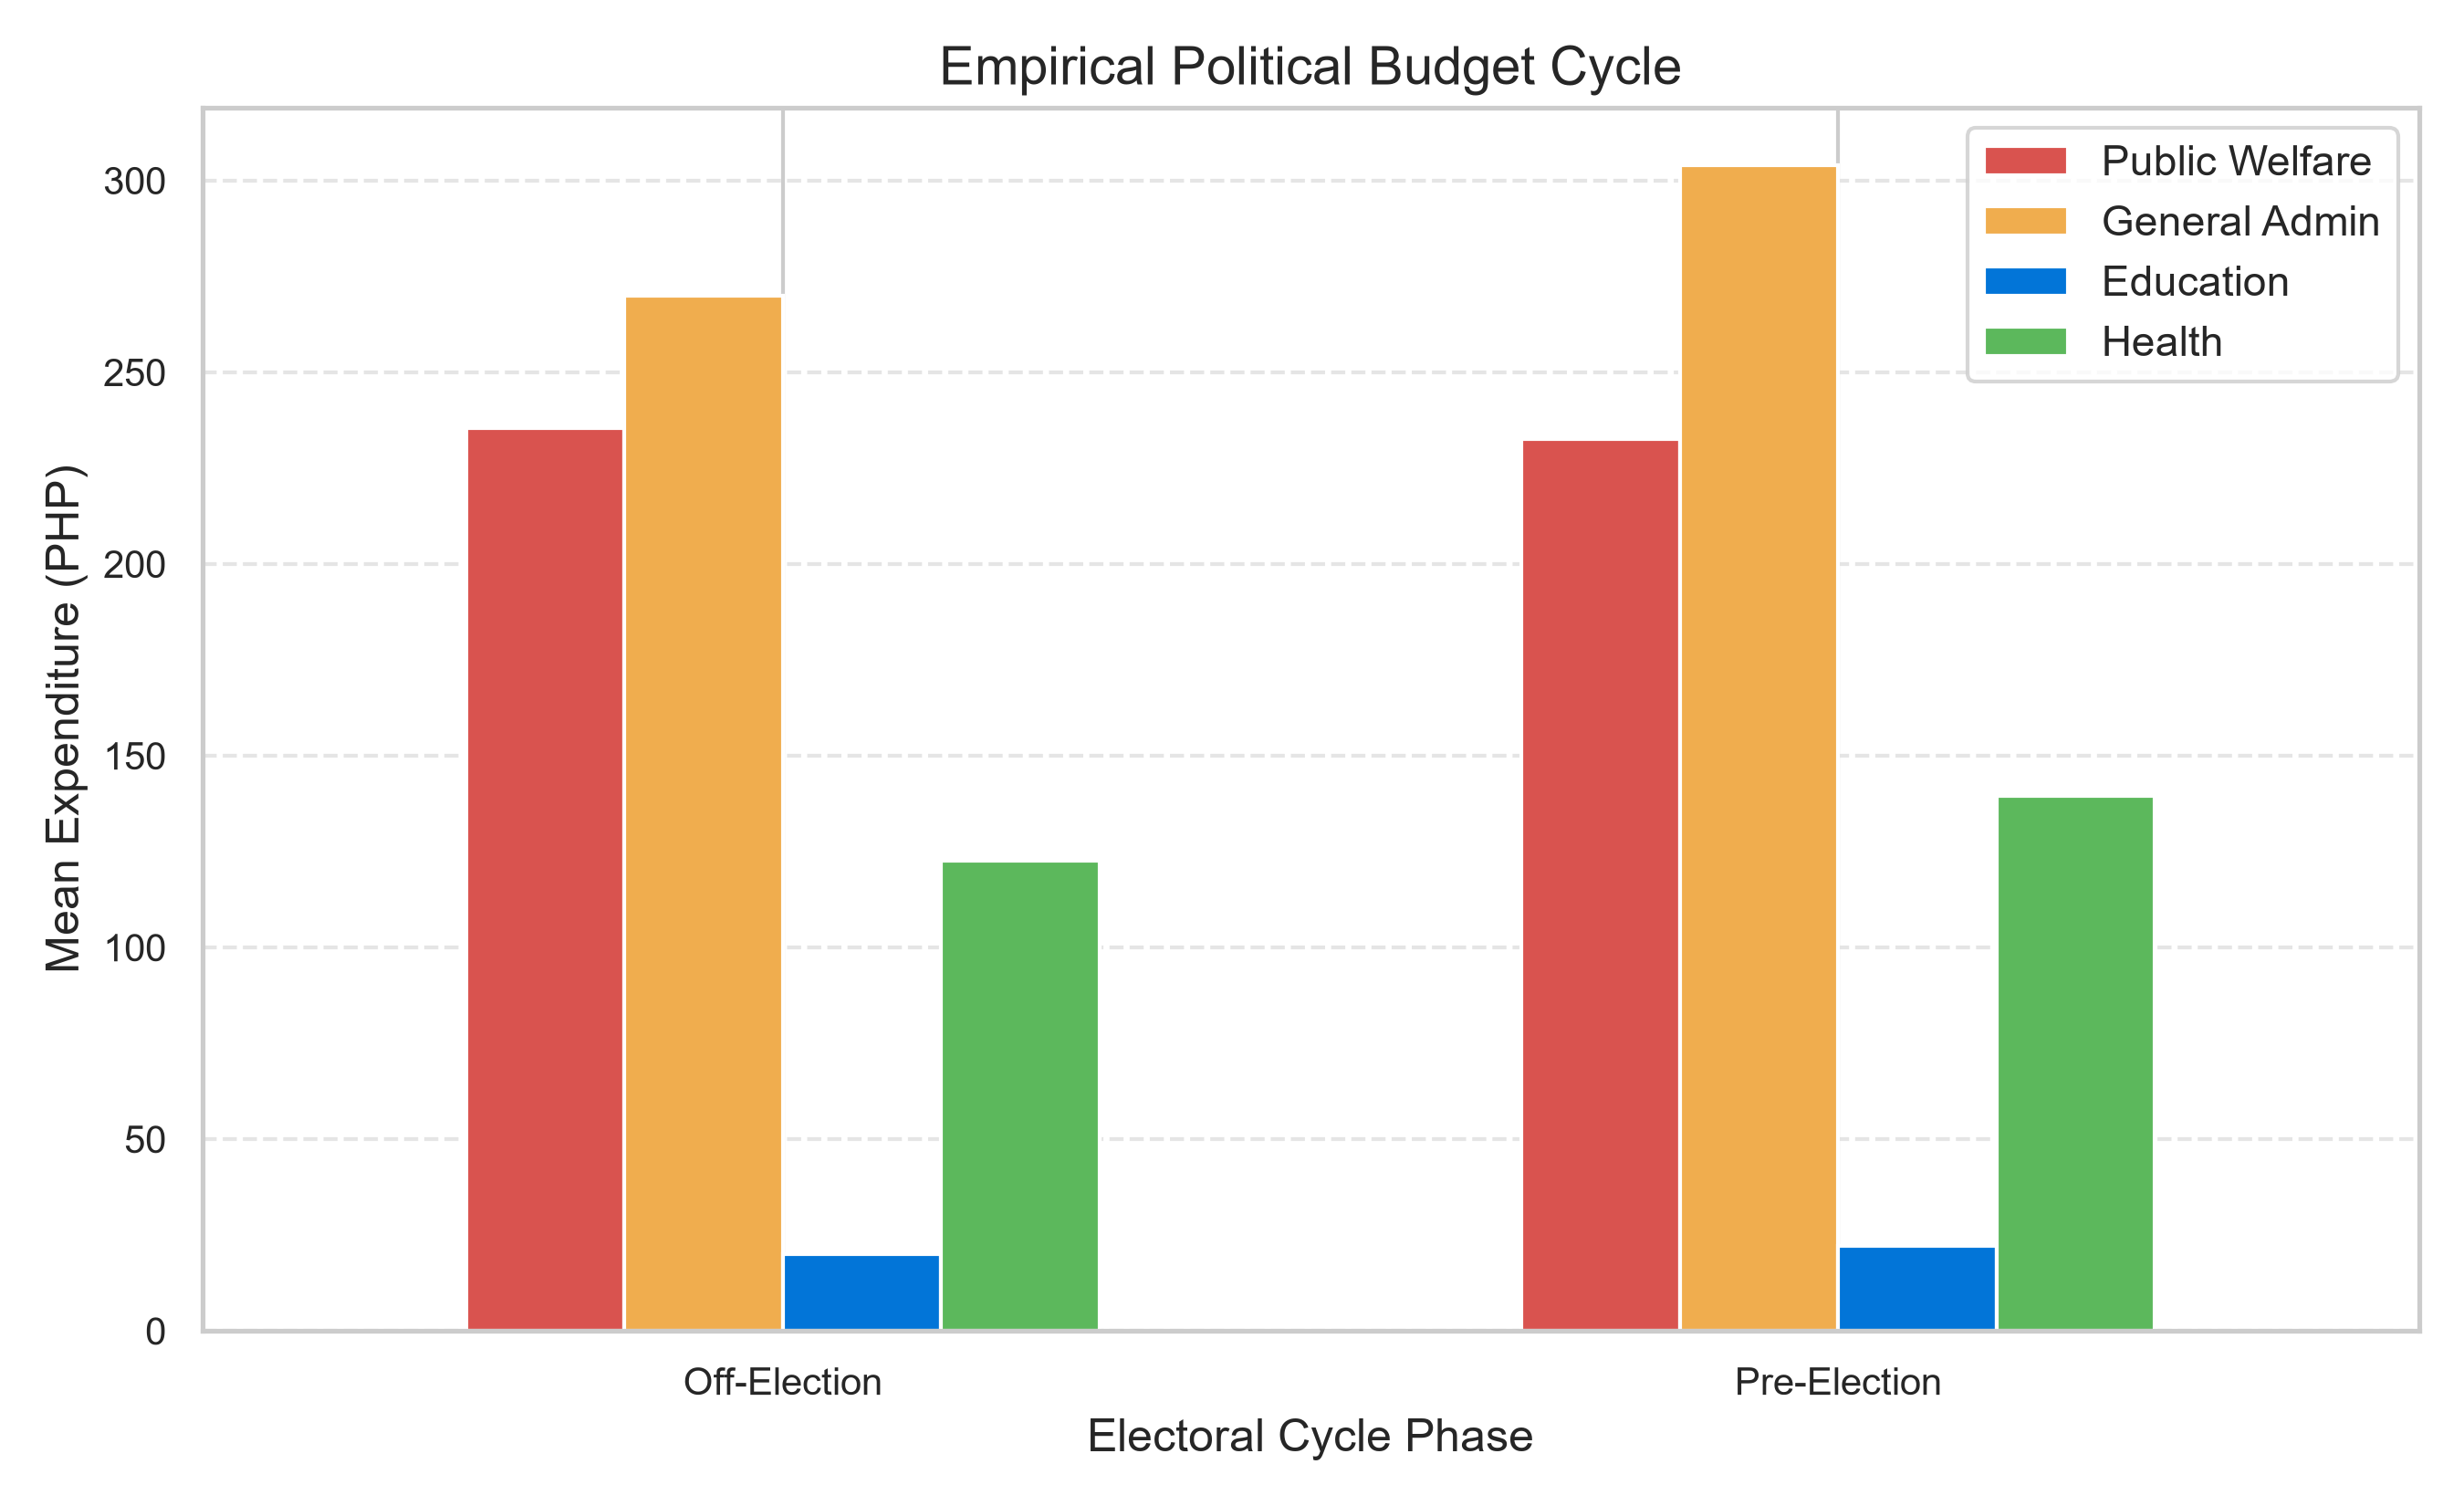
\includegraphics[width=0.9\linewidth]{../outputs/fig1_empirical_pbc.png}
\caption{Empirical Political Budget Cycle: Pre-Election Spending Surges}
\label{fig:pbc}
\end{figure}

\subsection{Deficit Distributions and Tail Risk}
Figure~\ref{fig:var} compares the deficit distributions under Scenarios A and B. Scenario A is shifted to the right, with a thicker tail. The 95\% VaR deficit rises from PHP 145.6M (Scenario B) to PHP 184.2M (Scenario A). The probability of single-period insolvency increases from 71.8\% to 76.9\%.

\begin{figure}[ht]
\centering
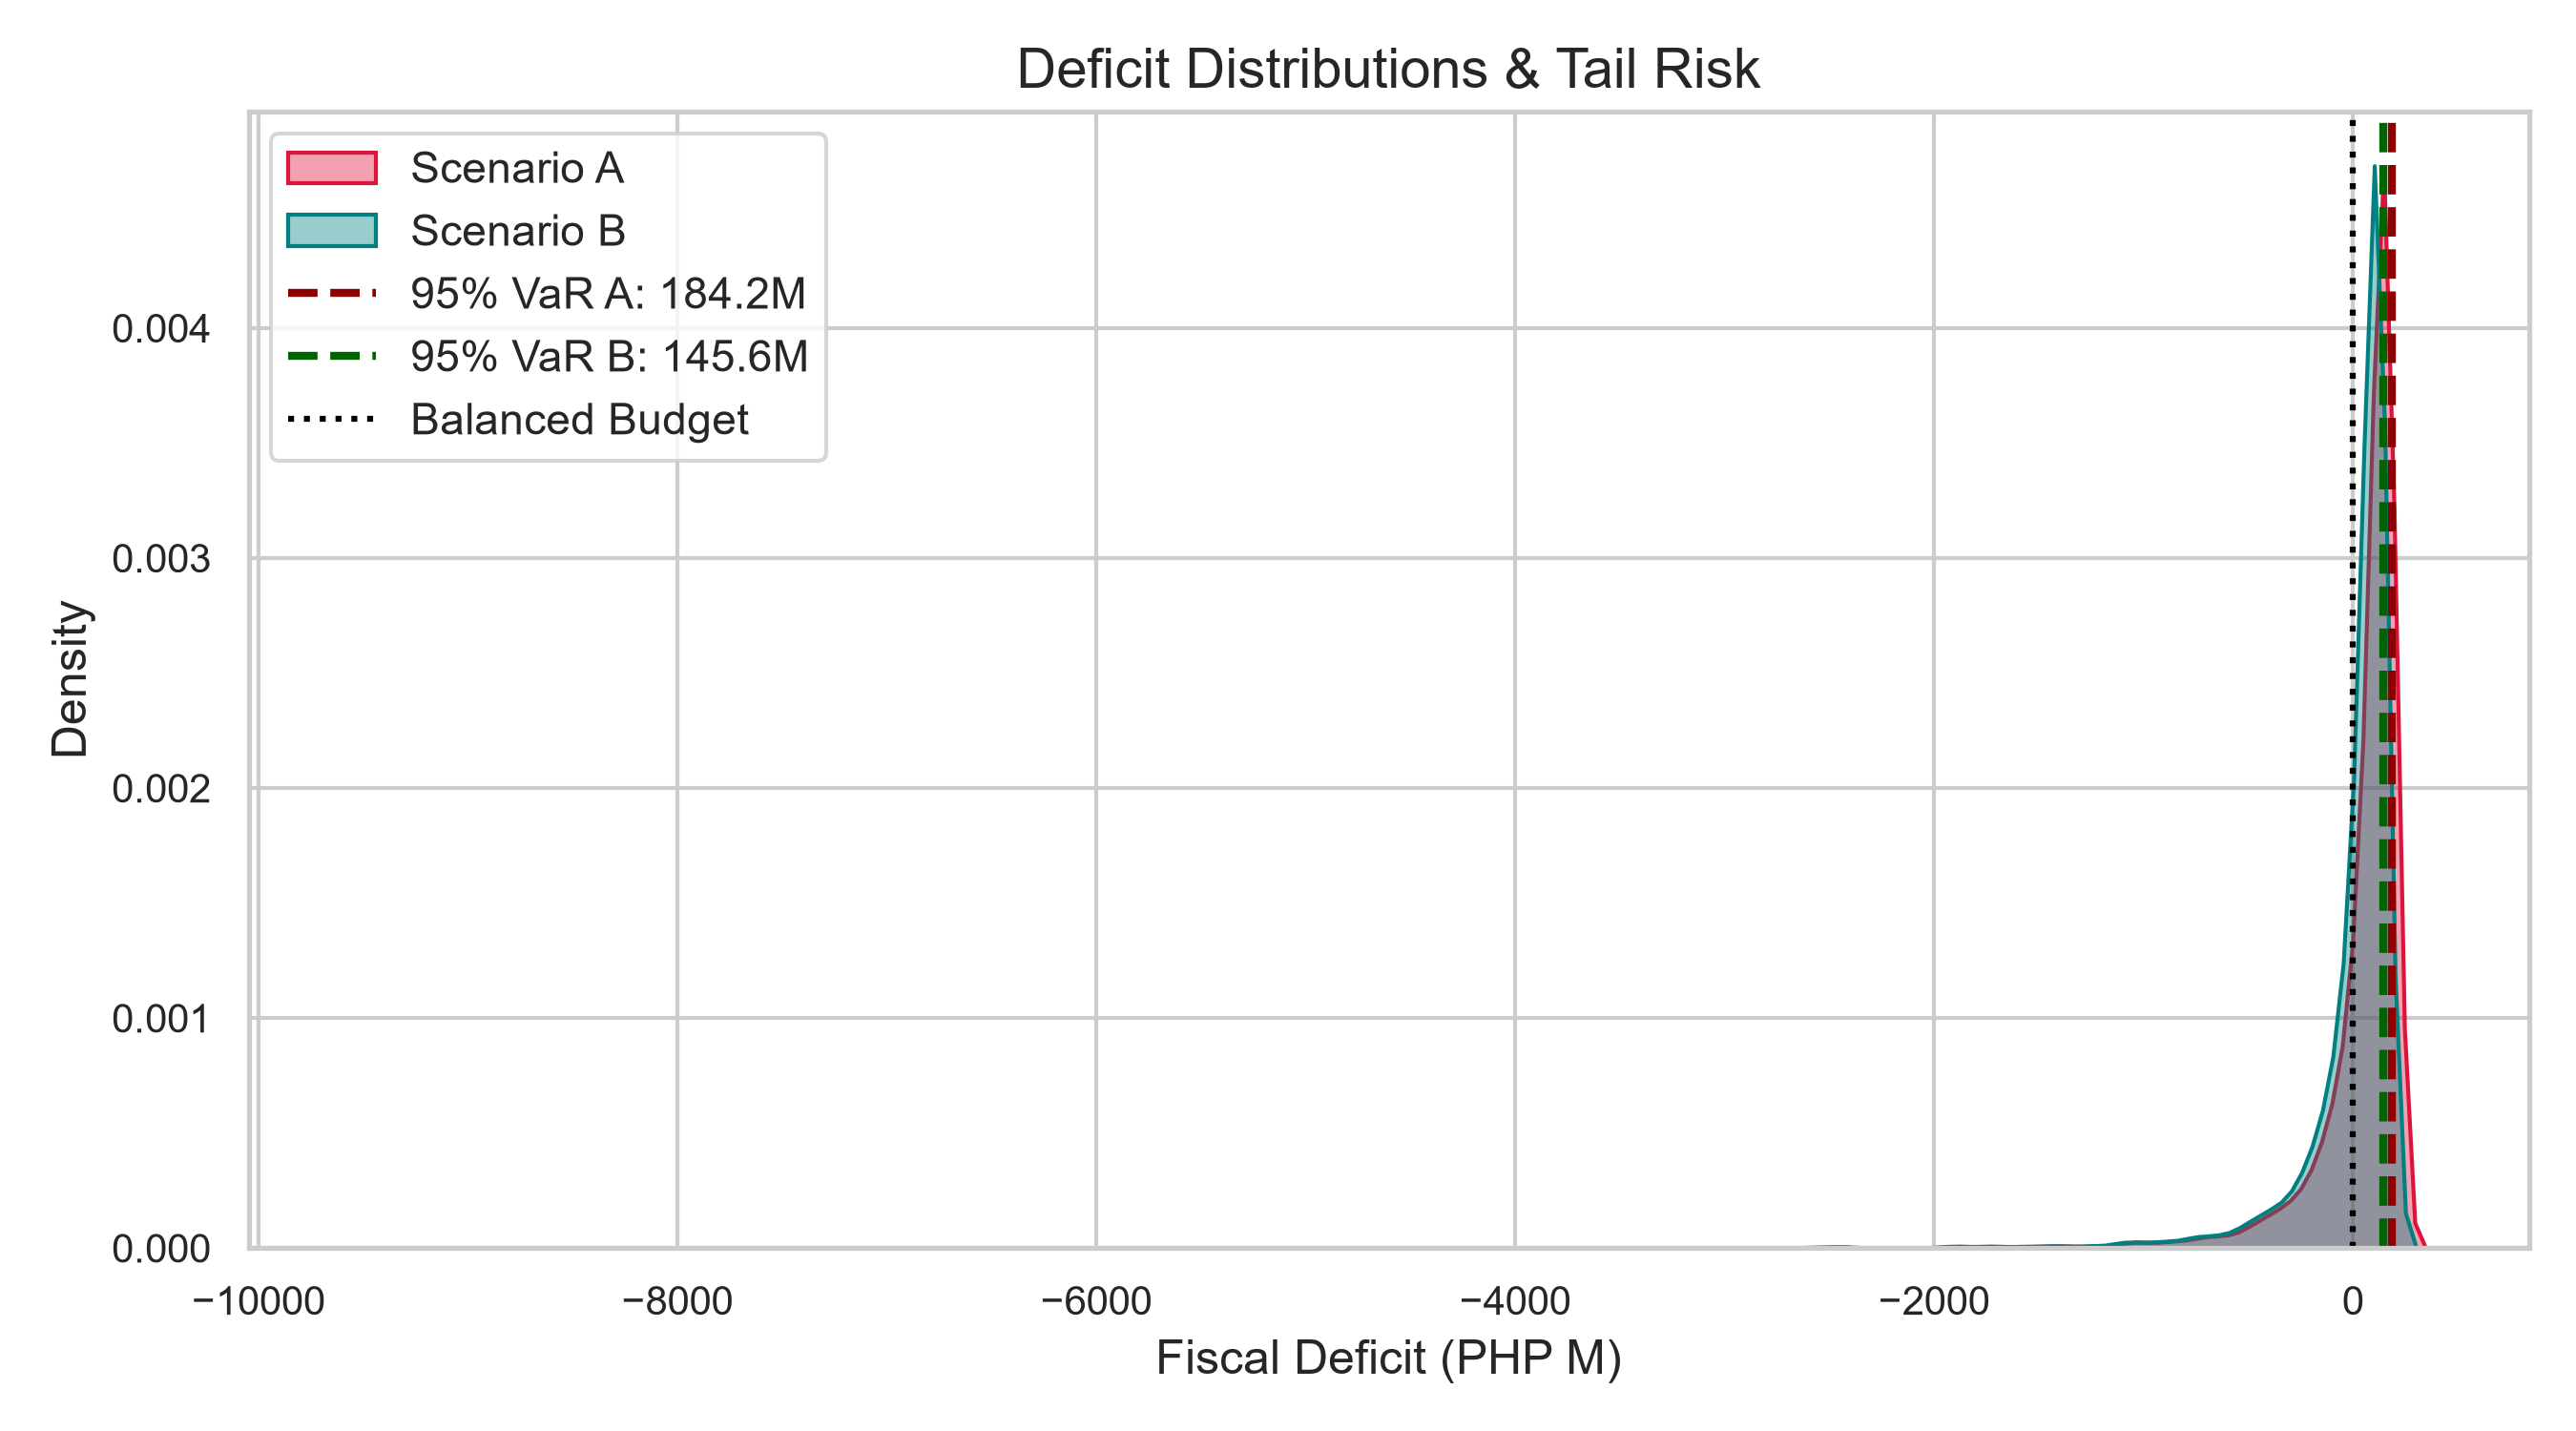
\includegraphics[width=0.9\linewidth]{../outputs/fig2_deficit_var_density.png}
\caption{Deficit Distributions and 95\% Value-at-Risk}
\label{fig:var}
\end{figure}

\subsection{Trade-Off Frontier}
Figure~\ref{fig:tradeoff} shows the trade-off between vote share and insolvency probability as the surge multiplier increases. Vote share remains virtually flat (around 0.51), while insolvency risk escalates sharply beyond a multiplier of 1.1. This illustrates the non-linearity and apparent inefficiency of patronage.

\begin{figure}[ht]
\centering
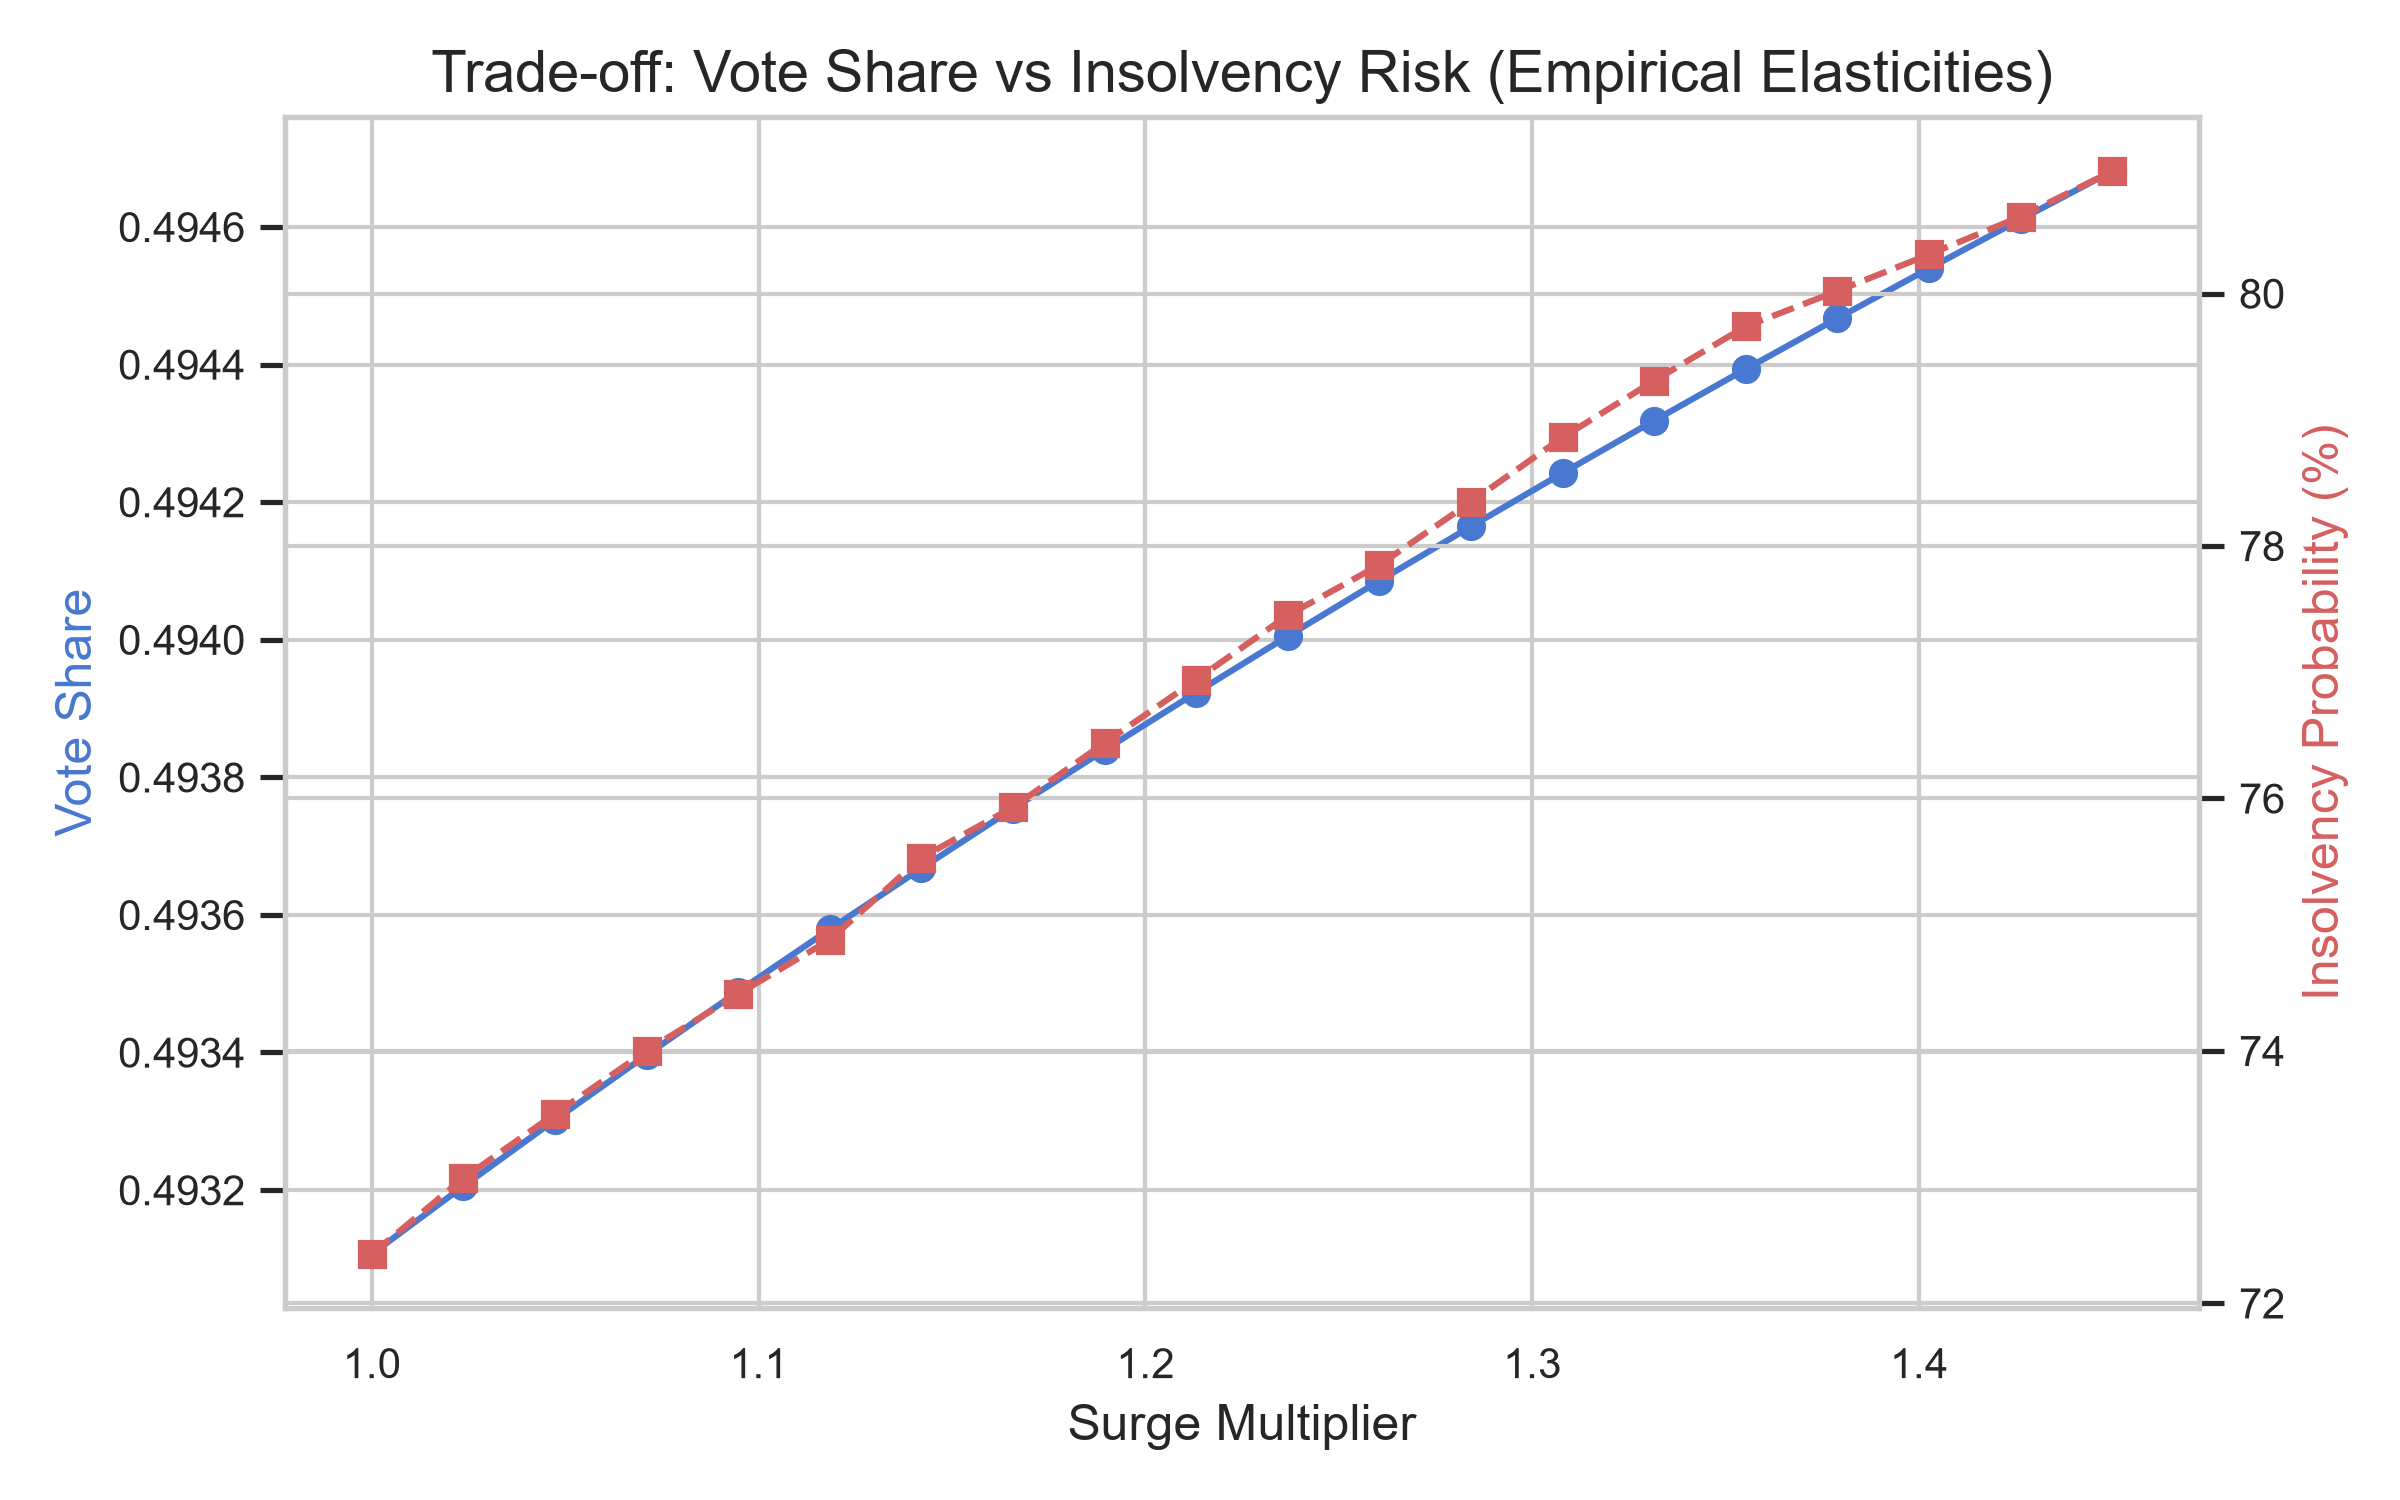
\includegraphics[width=0.9\linewidth]{../outputs/fig3_patronage_tradeoff_frontier.png}
\caption{Vote Share vs. Insolvency Risk Trade-Off}
\label{fig:tradeoff}
\end{figure}

\subsection{Sensitivity to Political Competition}
Figure~\ref{fig:heatmap} displays insolvency risk across combinations of the surge multiplier and the effective number of candidates (ENC). Higher competition (ENC) is associated with higher fiscal risk, as incumbents may feel pressured to spend more to fend off challengers. The heatmap suggests that risk is most acute when both competition and spending surges are high.

\begin{figure}[ht]
\centering
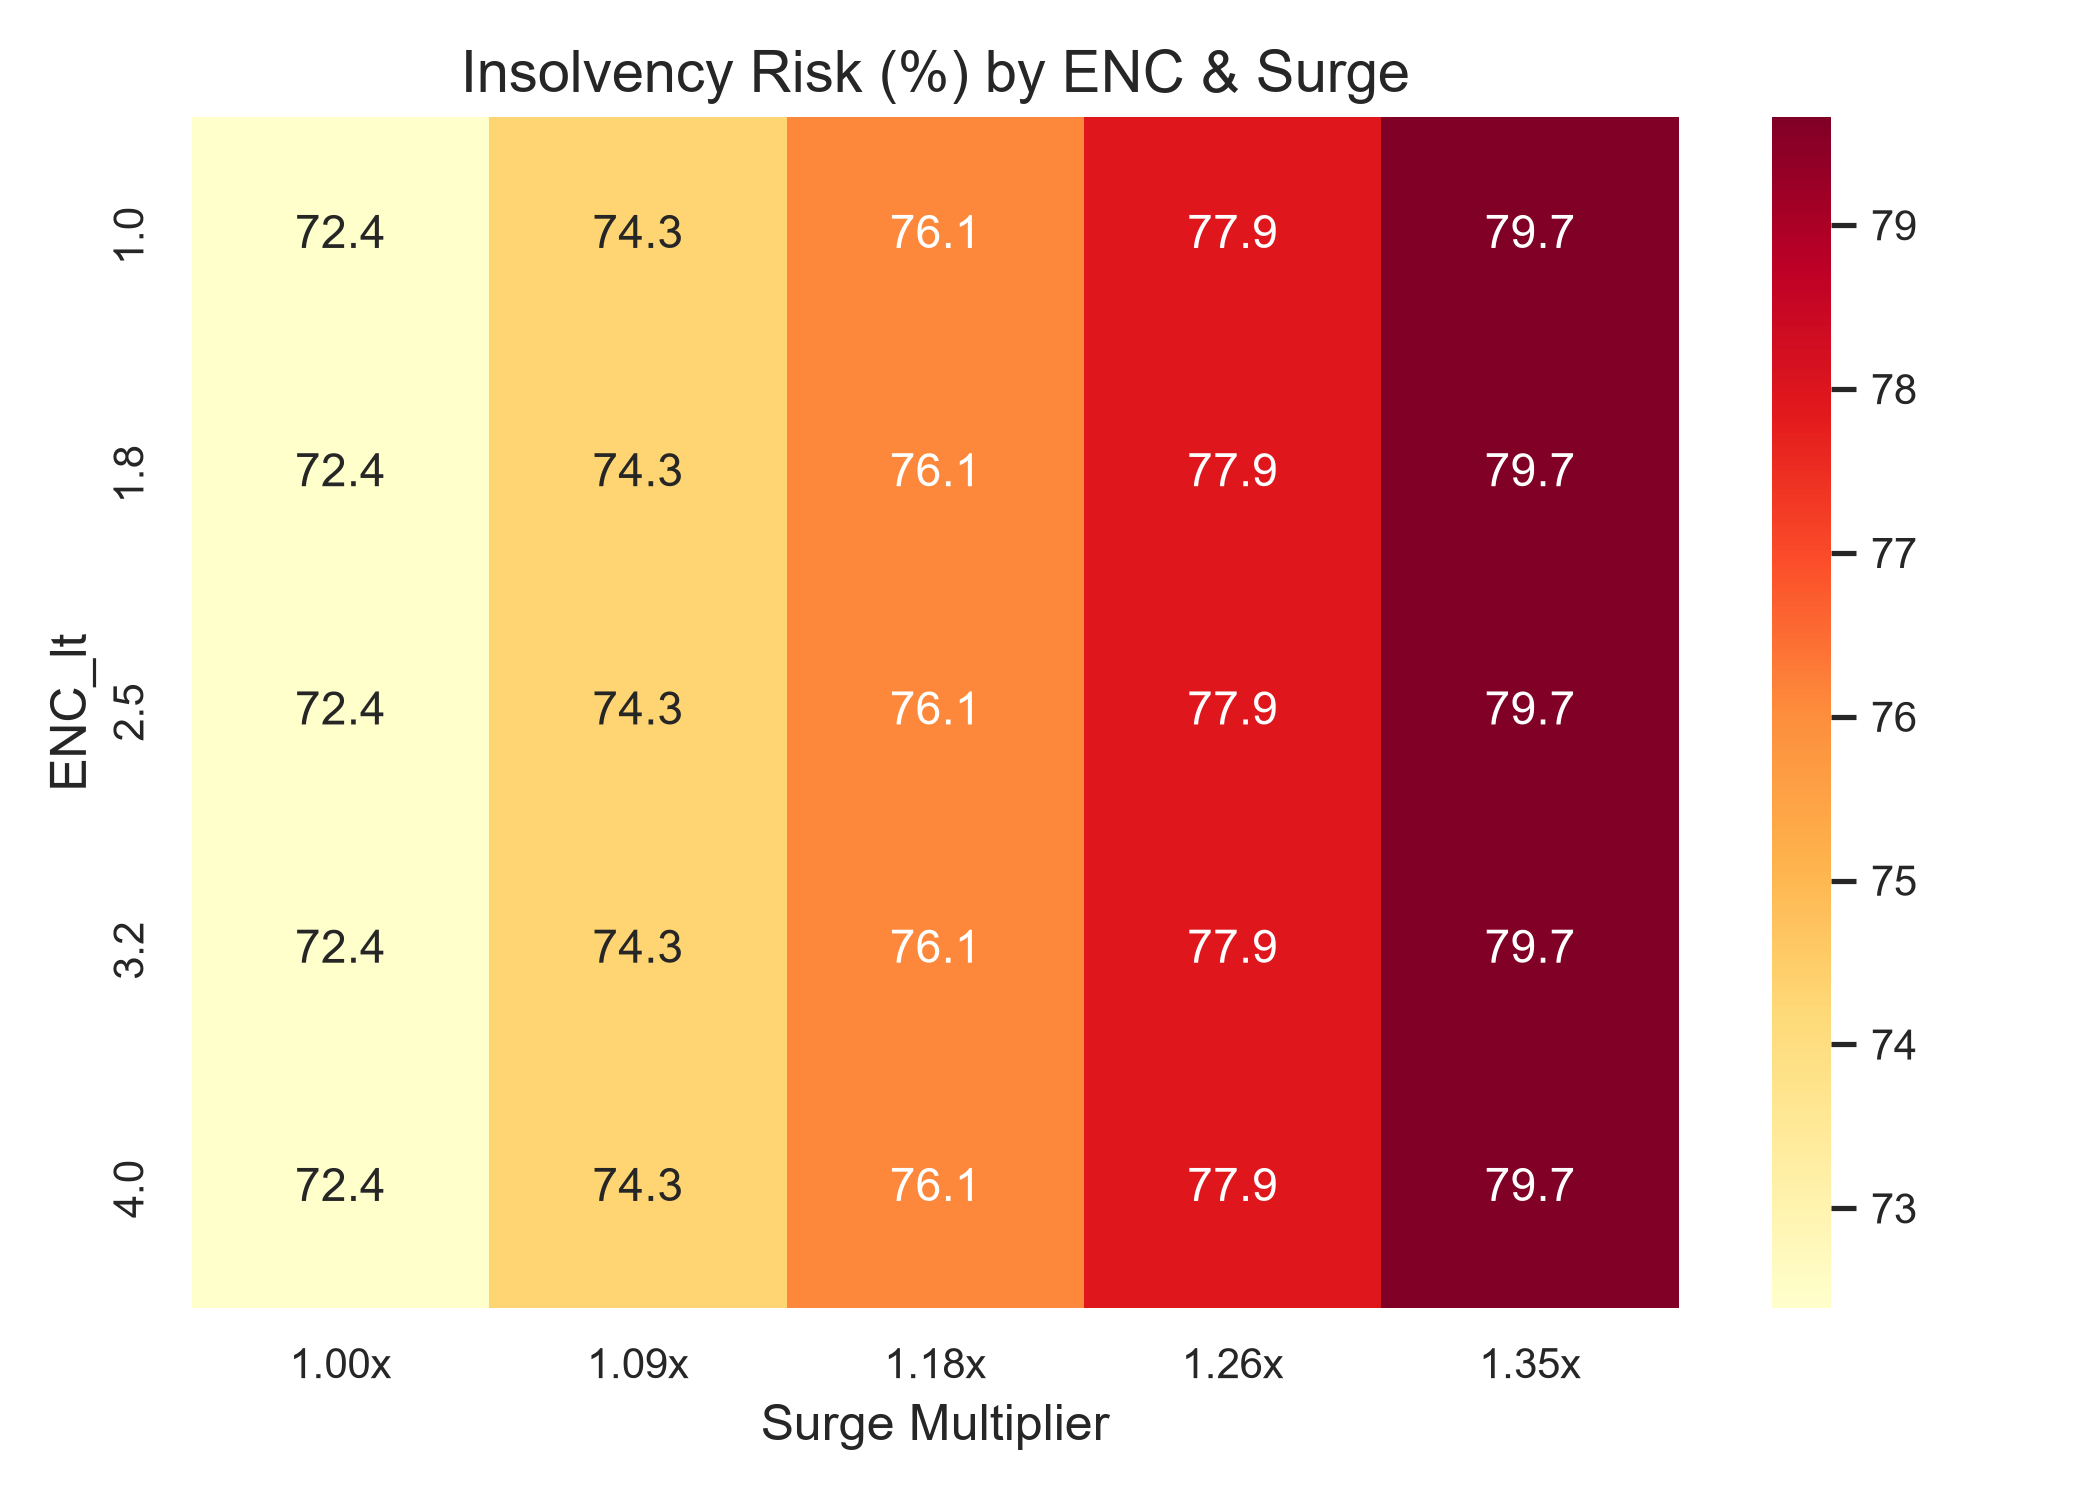
\includegraphics[width=0.9\linewidth]{../outputs/fig4_competition_risk_heatmap.png}
\caption{Insolvency Risk by ENC and Surge Multiplier}
\label{fig:heatmap}
\end{figure}

\subsection{Revenue Distributions}
Figure~\ref{fig:rev} shows the lognormal fits for local revenue and IRA, supporting the parametric assumptions used for simulating future revenue shocks.

\begin{figure}[ht]
\centering
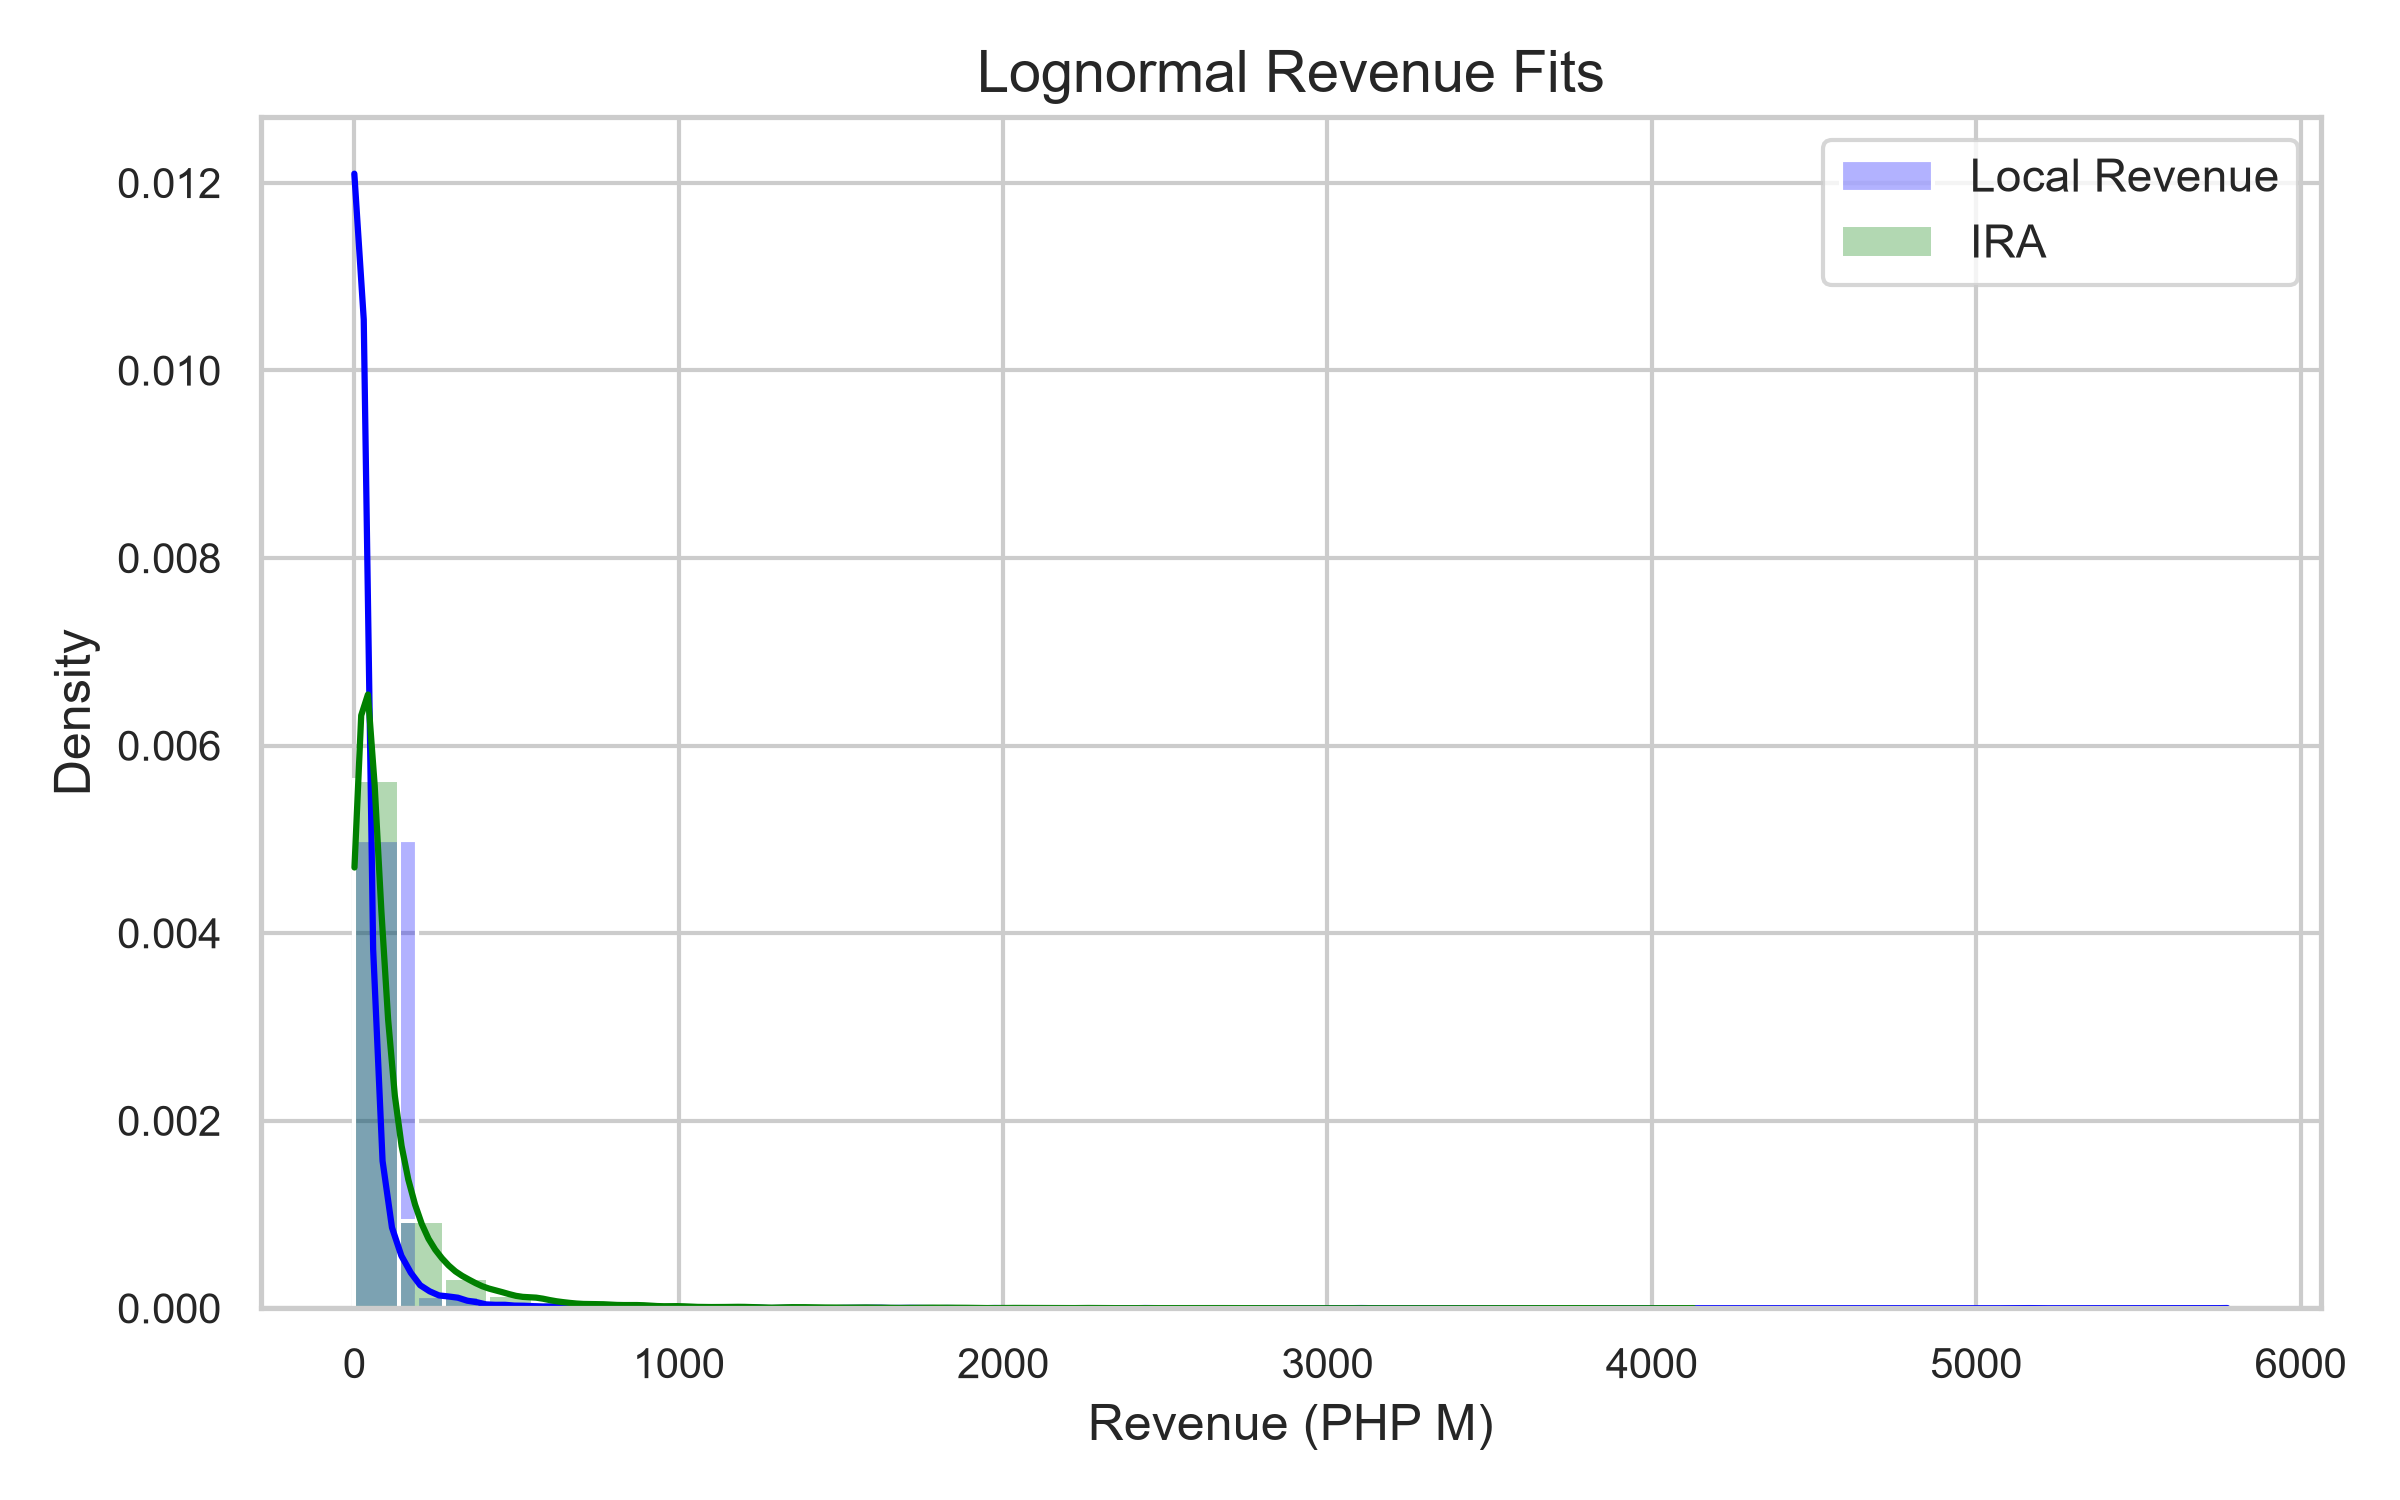
\includegraphics[width=0.9\linewidth]{../outputs/fig5_revenue_distributions.png}
\caption{Lognormal Revenue Fits}
\label{fig:rev}
\end{figure}

\subsection{Cumulative Deficit Trajectories}
Figure~\ref{fig:cum} illustrates 50 stochastic 10-year cumulative deficit paths under Scenario A. The mean cumulative deficit grows steadily, and the probability of cumulative insolvency (73.8\%) is substantially higher than under Scenario B (54.9\%).

\begin{figure}[ht]
\centering
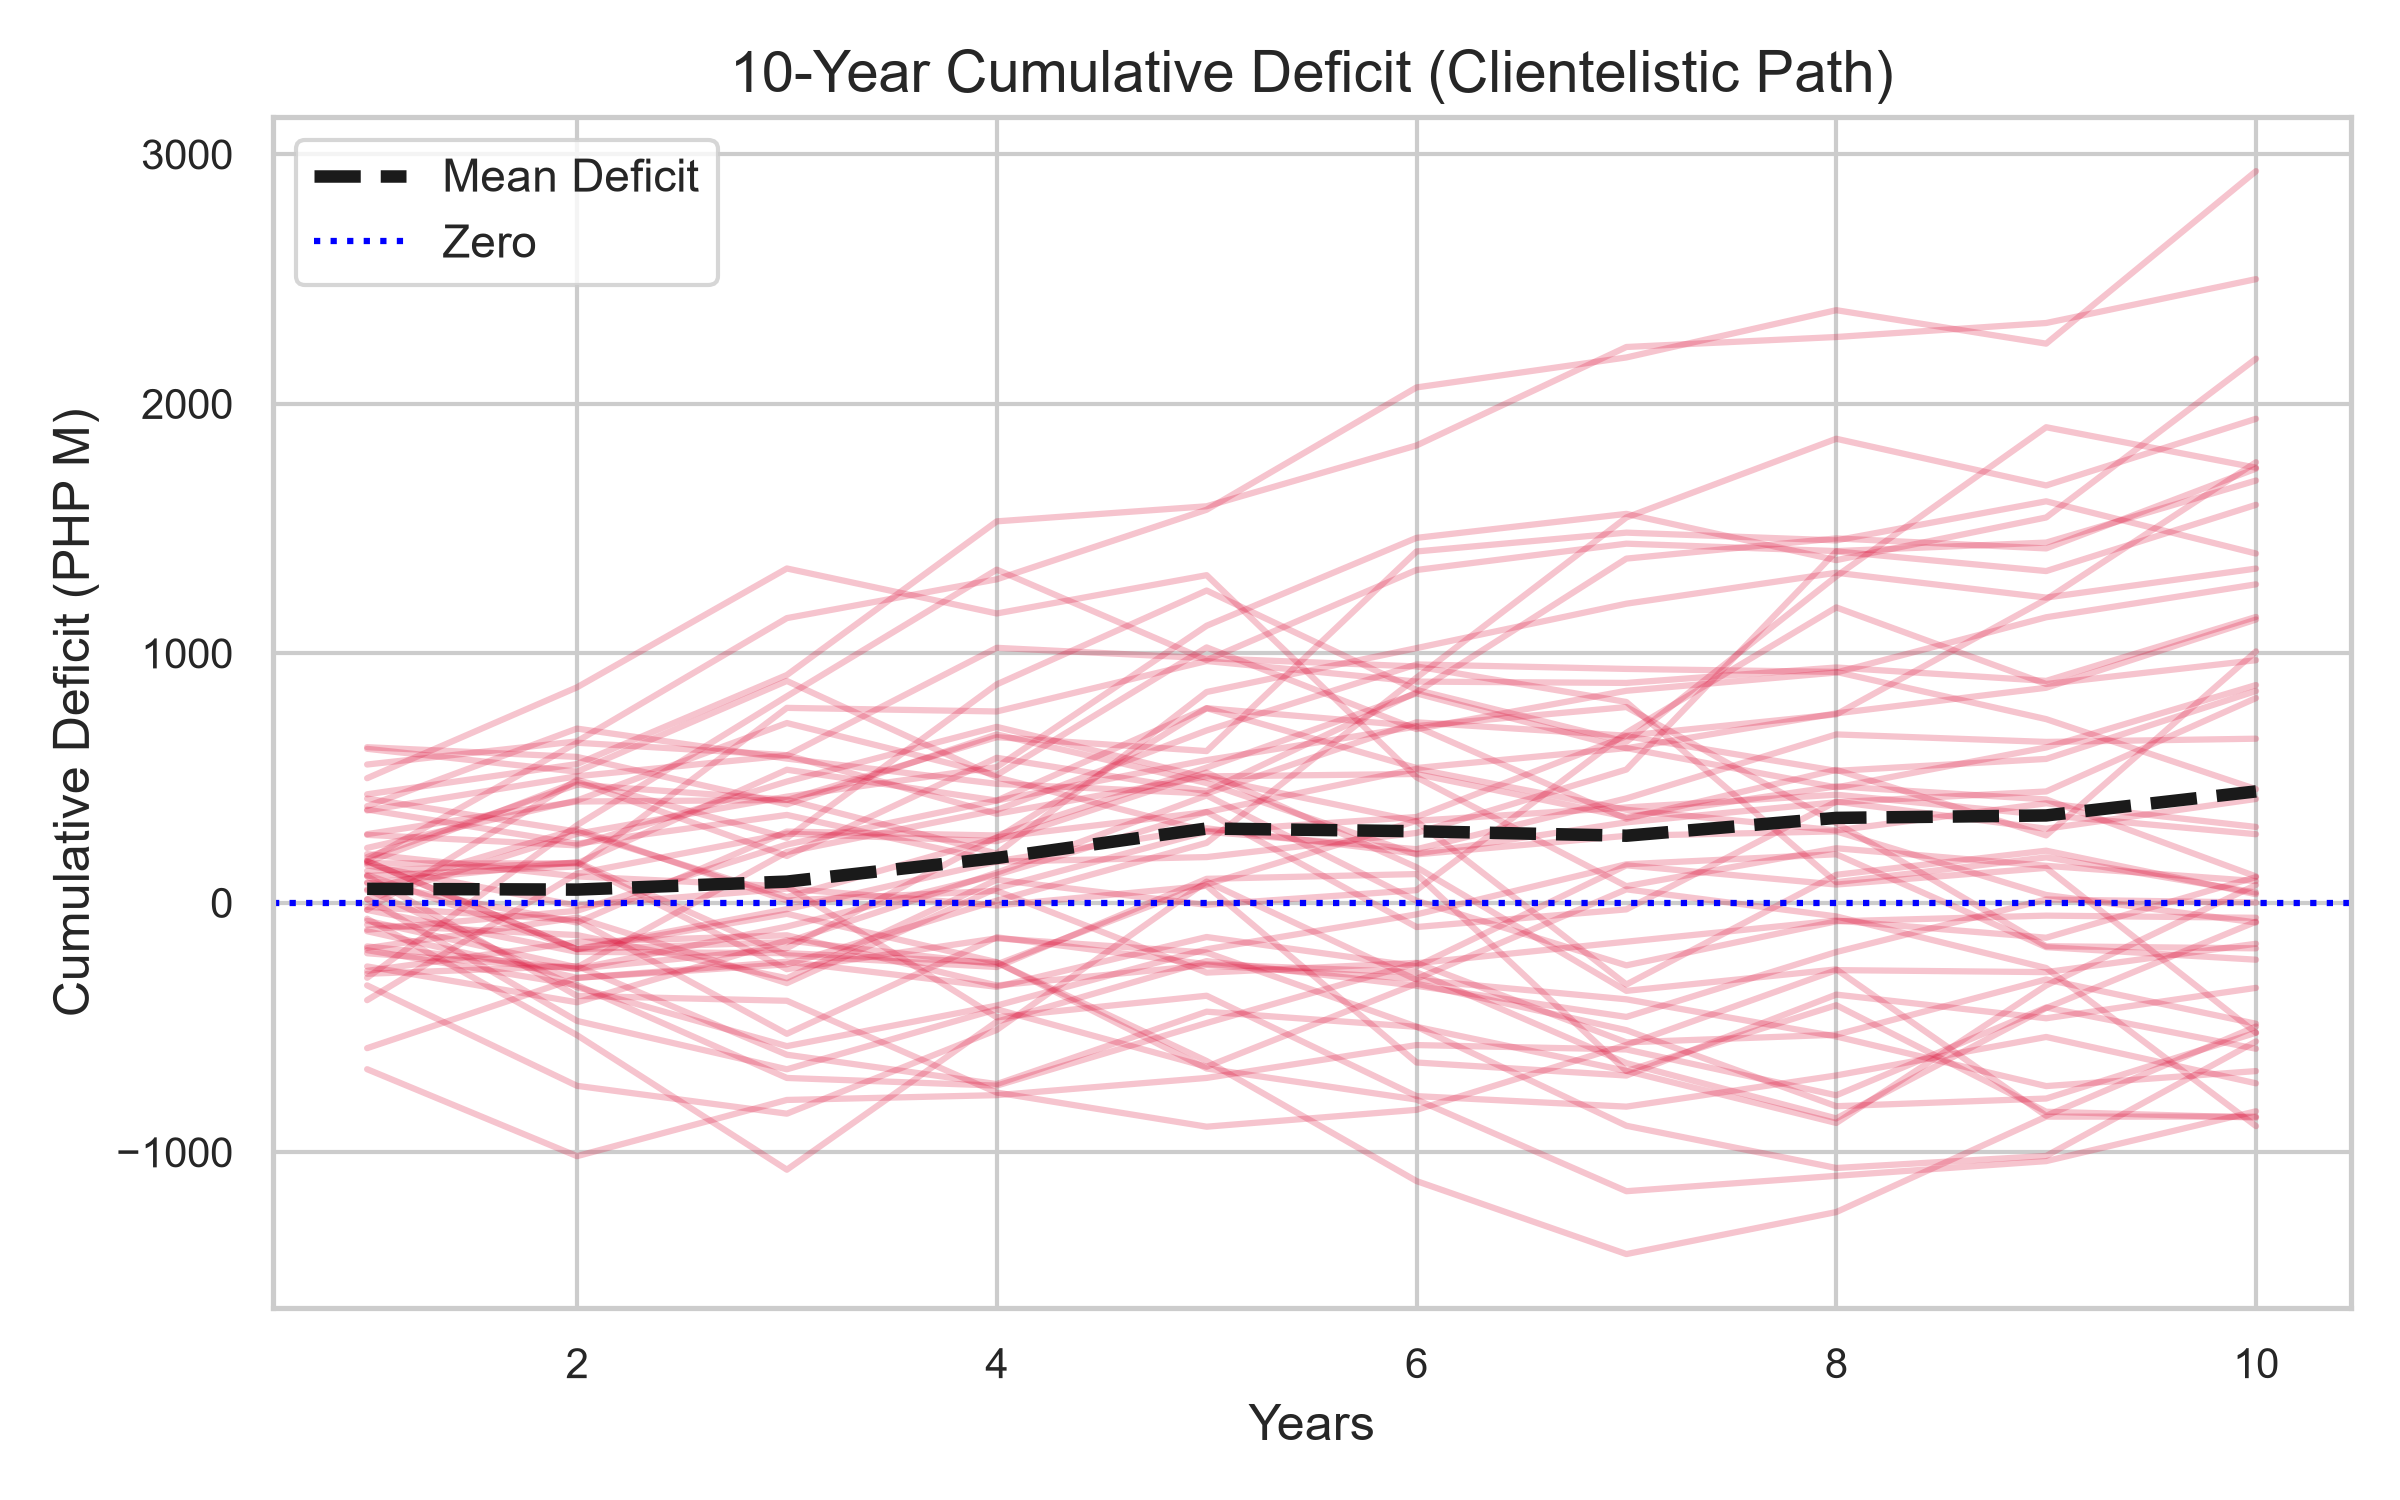
\includegraphics[width=0.9\linewidth]{../outputs/fig6_10yr_stochastic_trajectories.png}
\caption{10-Year Cumulative Deficit Trajectories (Clientelistic Path)}
\label{fig:cum}
\end{figure}

\subsection{Diagnostic Plots}
Figure~\ref{fig:diag} provides diagnostic scatter and histogram plots. The upper-left panel shows the distribution of simulated income; the upper-right plots the deficit-to-income ratio. The lower panels show no clear relationship between vote share and fiscal risk (correlation coefficient $-0.02$), nor between income and deficit ($\rho=-0.03$), suggesting that the electoral cost is largely independent of fiscal condition. The confidence interval around the vote-share difference includes zero and small positive/negative values; thus, while we cannot reject the hypothesis of a zero effect, the point estimate is negative.

\begin{figure}[ht]
\centering
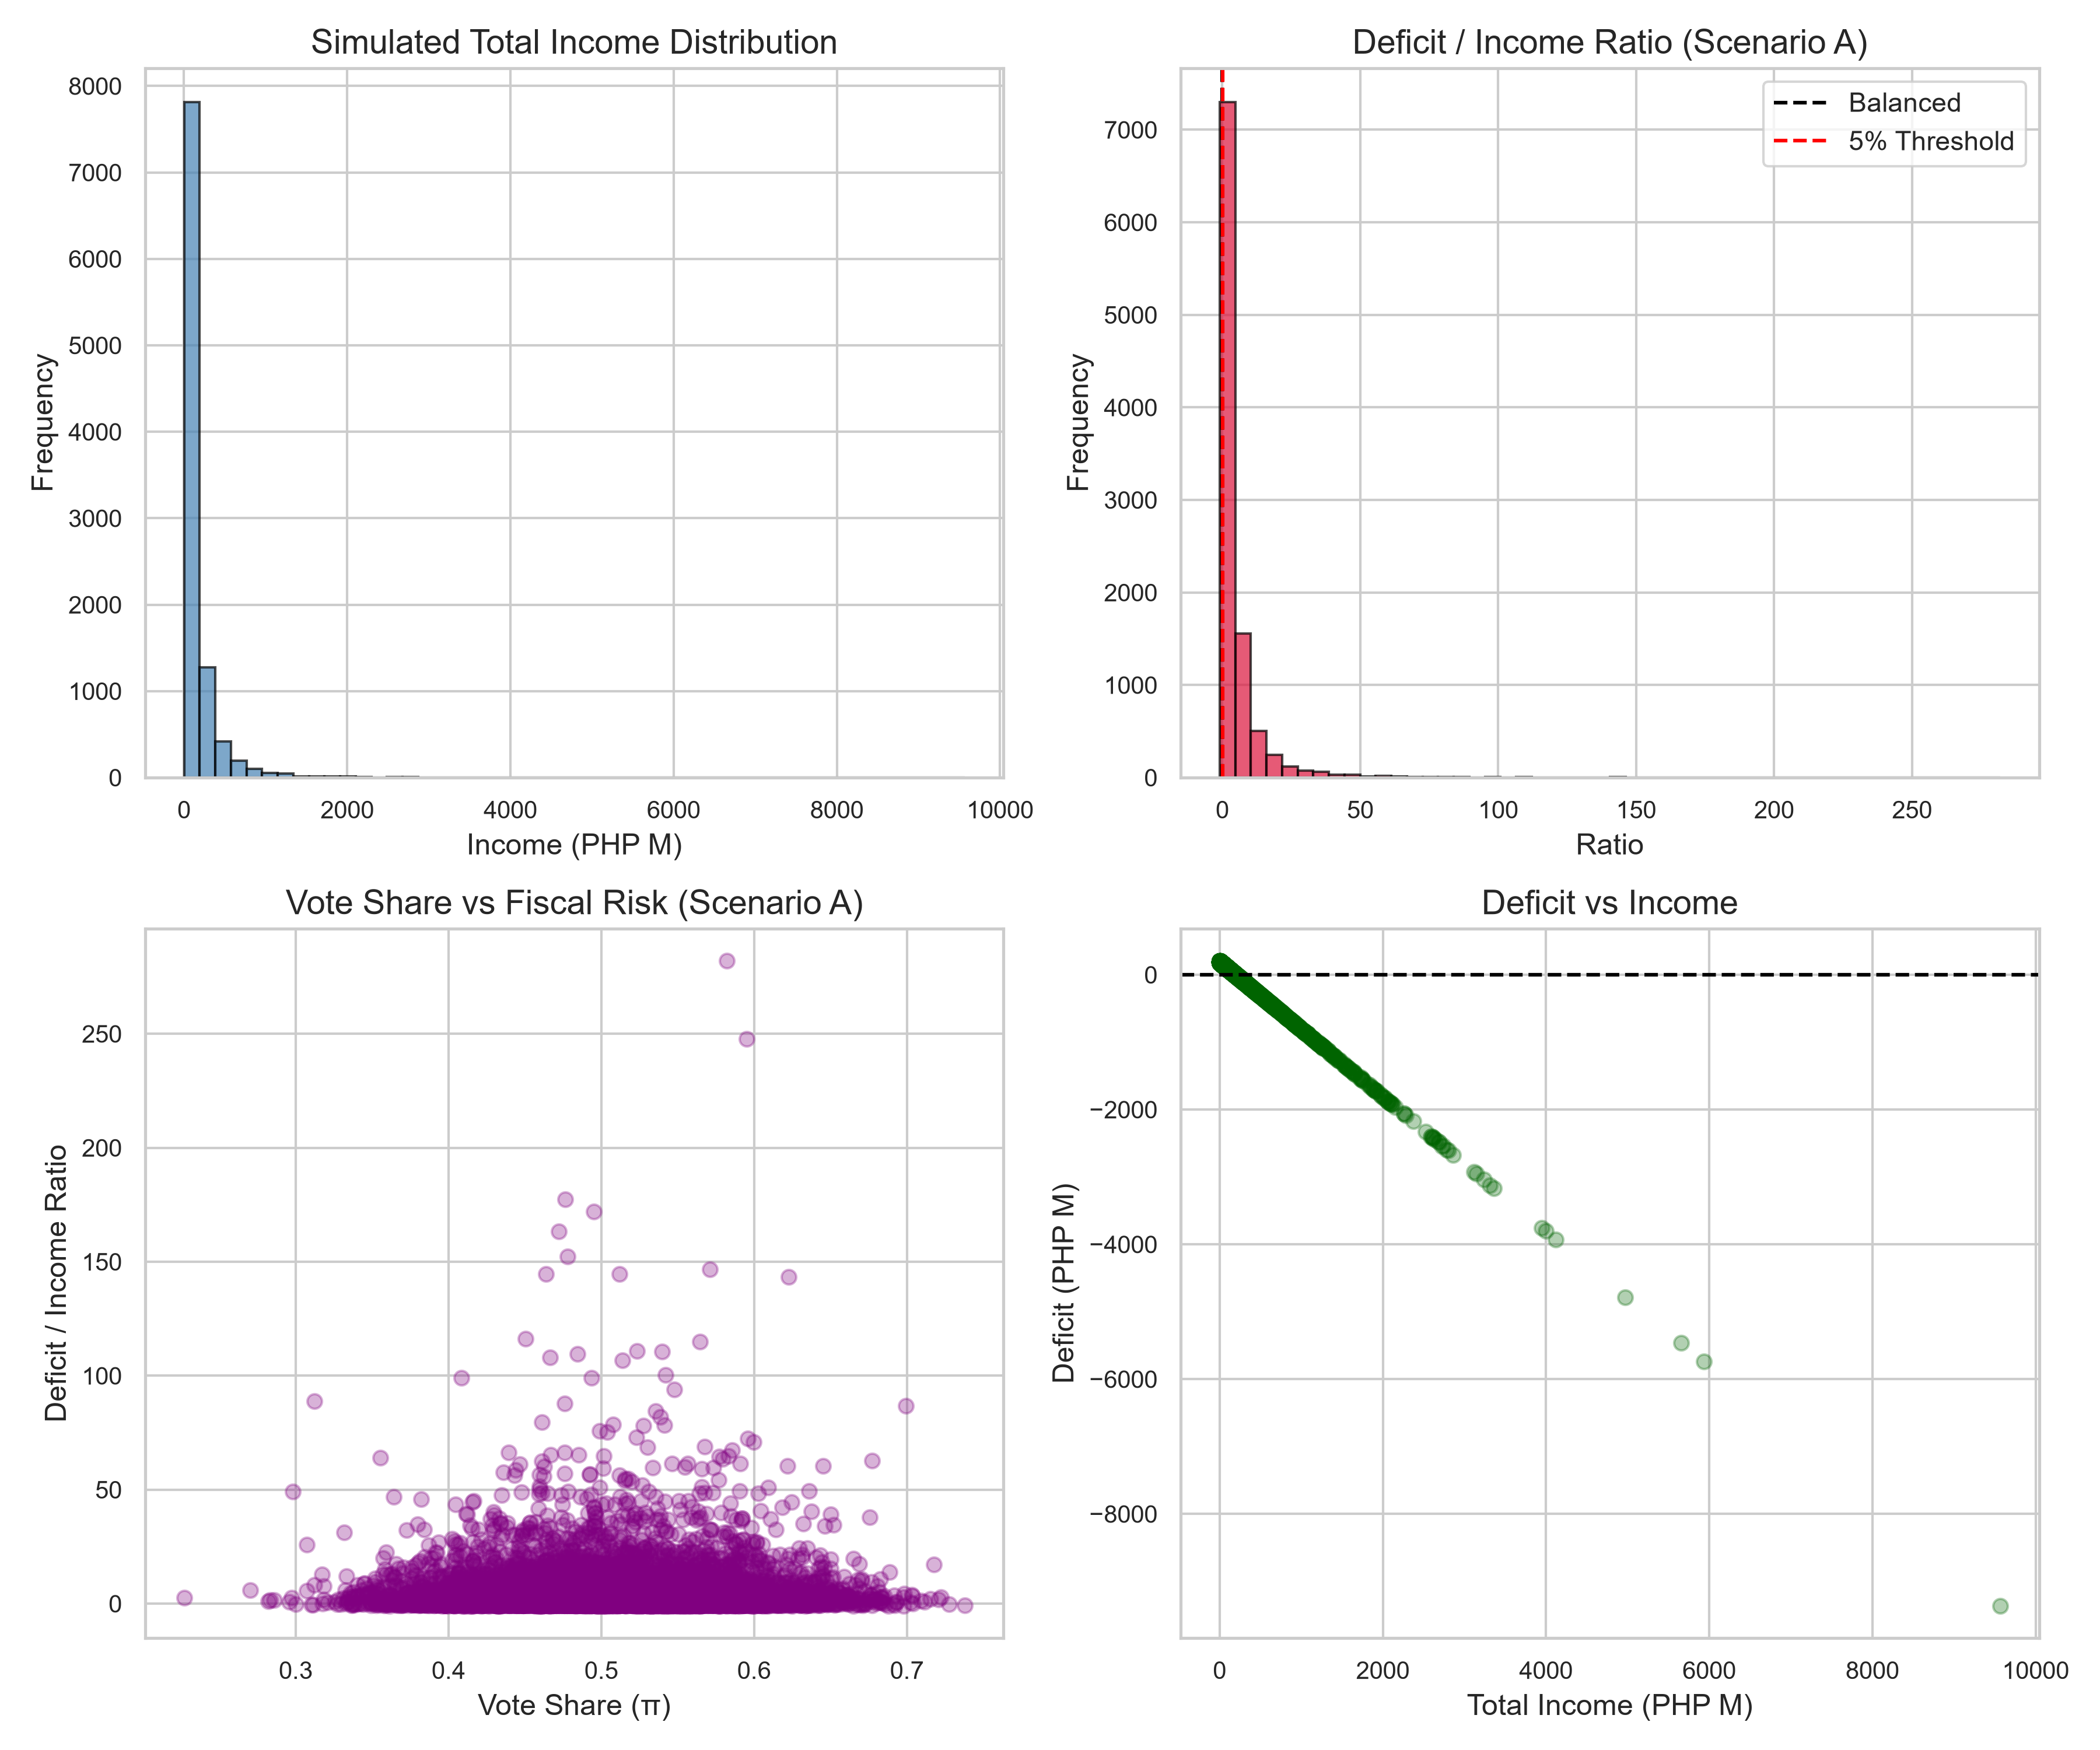
\includegraphics[width=0.9\linewidth]{../outputs/fig7_diagnostics.png}
\caption{Diagnostic Plots}
\label{fig:diag}
\end{figure}

\subsection{Summary of Key Quantities}
Table~\ref{tab:main} summarises the main simulation outputs. Scenario A increases total expenditure by PHP 37.64M, turns a surplus into a deficit, raises 95\% VaR by PHP 38.64M, and increases 10-year cumulative insolvency probability by 18.9 percentage points---all while delivering a (non-significant) \emph{lower} vote share.

\begin{table}[ht]
\centering
\caption{Monte Carlo Simulation Summary Results}
\label{tab:main}
\small
\begin{tabular}{lcc}
\toprule
Metric & Scenario A & Scenario B \\
\midrule
Expenditure (PHP M) & 192.53 & 154.89 \\
Deficit/Surplus (PHP M)$^a$ & 34.30 & -3.34 \\
Insolvency Probability (1-year) & 0.769 & 0.718 \\
95\% VaR Deficit (PHP M) & 184.23 & 145.59 \\
Mean Vote Share ($\pi$) & 0.508 & 0.509 \\
Vote Share Std. Dev. & 0.0645 & 0.0658 \\
10-Year Cumulative Insolvency Prob. & 0.738 & 0.549 \\
\bottomrule
\end{tabular}
\par\smallskip
\footnotesize{$^a$ Positive values indicate a deficit; negative values indicate a surplus.}
\end{table}

\section{Discussion}

Our results offer three main insights. First, they are consistent with the view that pre-election clientelism is electorally inefficient: the marginal vote return of discretionary spending is close to zero, and reallocating funds toward education and health yields a slightly higher vote share. This aligns with the ``political budget cycle'' literature that finds spending surges are often wasteful \cite{brender2005political}. However, the estimated vote-share effect is not precisely estimated; the confidence interval includes both small positive and negative values, so we cannot claim that patronage has no effect---only that any effect is likely small and imprecisely measured.

Second, the fiscal consequences appear severe. The ``incumbent tax'' materialises as a structural reversal from surplus to deficit, and a dramatic increase in tail-risk exposure. Philippine LGUs are heavily dependent on IRA transfers; a revenue shortfall coupled with pre-election overspending could trigger insolvency and hamper essential service delivery in the post-election period.

Third, the 10-year cumulative insolvency probability under the clientelistic path (73.8\%) is alarming. This highlights the importance of dynamic fiscal guardrails, such as multi-year budget ceilings and stress-testing requirements for LGUs.

We also conducted several sensitivity checks. Re-estimating the voter elasticity model without winsorizing the top 1\% of fiscal variables did not materially change the coefficients (education remained the most positive; public welfare remained small). Treating zeros in sectoral expenditures as zero rather than missing also yielded similar point estimates, though standard errors increased slightly. Varying the revenue correlation $\rho$ between 0.3 and 0.6 altered the insolvency probabilities by less than 2 percentage points. Thus, the qualitative conclusions are robust to these alternative specifications.

However, several limitations should be acknowledged. Our model assumes that the surge multiplier is drawn independently each year, ignoring potential persistence or learning by incumbents. We also treat the expenditure allocation shares as fixed, though in reality they may vary. The fixed-effects voter elasticity model may suffer from reverse causality if lagged vote shares influence future spending; we do not address endogeneity beyond including LGU fixed effects. Moreover, the model explains only about 21\% of the within-LGU variation in vote share, so unobserved factors likely play a large role in electoral outcomes.

Future work could incorporate dynamic programming to model optimal spending decisions under uncertainty, or use instrumental variables to strengthen causal identification.

\section{Conclusion}

This paper has developed a stochastic simulation framework to assess the electoral and fiscal implications of pre-election clientelism in Philippine LGUs. Using 31 years of panel data and a Monte Carlo engine calibrated to empirical elasticities, we find that the typical patronage-driven surge yields at most small electoral returns while imposing substantial fiscal costs: a reversal from surplus to deficit, elevated insolvency risk, and enlarged tail-risk exposure. The evidence is consistent with the notion of an ``incumbent tax''—a fiscal burden that incumbents appear to impose on their own jurisdictions with little clear electoral compensation.

The policy implications are clear. Regulatory agencies (DBM, BLGF, DILG) should:

\begin{enumerate}
\item Impose pre-election discretionary spending ceilings (e.g., limiting total expenditure growth to 5\% above the prior year's level).
\item Mandate fiscal stress tests for LGUs with high local revenue volatility or high IRA dependence.
\item Encourage a shift toward human-capital investments (education and health) by linking IRA releases to compliance with sectoral spending floors.
\end{enumerate}

The incumbent tax pattern is empirically robust and policy-relevant, even if the underlying electoral mechanism warrants further identification work. Our results provide a compelling evidence base for reforming local fiscal governance in the Philippines and offer a template for similar analyses in other developing democracies. By aligning with SDG 16 (inclusive institutions) and SDG 1/3/4 (poverty, health, education), this work contributes to the broader agenda of sustainable and accountable governance.

\clearpage
\bibliographystyle{plain}
\begin{thebibliography}{99}

\bibitem{akhmedov2004opportunistic}
Akhmedov, A., \& Zhuravskaya, E. (2004). Opportunistic political cycles: Test in a young democracy setting. \emph{Quarterly Journal of Economics}, 119(4), 1301--1338.

\bibitem{brender2005political}
Brender, A., \& Drazen, A. (2005). Political budget cycles in new versus established democracies. \emph{Journal of Monetary Economics}, 52(7), 1271--1295.

\bibitem{capuno2016patronage}
Capuno, J. J. (2016). Patronage, pork barrel, and political budget cycles in the Philippines. \emph{Philippine Review of Economics}, 53(1), 1--24.

\bibitem{drazen2006electoral}
Drazen, A., \& Eslava, M. (2006). Electoral manipulation via voter-friendly spending: Theory and evidence. \emph{Journal of Development Economics}, 88(1), 1--18.

\bibitem{golden2014distributive}
Golden, M. A., \& Min, B. (2014). Distributive politics around the world. \emph{Annual Review of Political Science}, 16, 73--99.

\bibitem{keefer2005electoral}
Keefer, P., \& Khemani, S. (2005). Democracy, public expenditures, and the poor. \emph{World Bank Research Observer}, 20(1), 1--27.

\bibitem{llanto2016local}
Llanto, G. M., \& Ortiz, M. K. P. (2016). Local government fiscal and institutional constraints. \emph{Philippine Institute for Development Studies Discussion Paper}, 2016-21.

\bibitem{glasserman2003monte}
Glasserman, P. (2003). \emph{Monte Carlo Methods in Financial Engineering}. Springer.

\bibitem{shi2006political}
Shi, M., \& Svensson, J. (2006). Political budget cycles: A review. \emph{Journal of Economic Surveys}, 20(3), 357--381.

\bibitem{brollo2013political}
Brollo, F., Nannicini, T., Perotti, R., \& Tabellini, G. (2013). The political resource curse. \emph{American Economic Review}, 103(5), 1759--1796.

\bibitem{diermeier2007political}
Diermeier, D., \& Feddersen, T. J. (2007). Elections and fiscal policy. \emph{Journal of Political Economy}, 115(2), 234--267.

\bibitem{ferraz2008electoral}
Ferraz, C., \& Finan, F. (2008). Exposing corrupt politicians: The effects of Brazil's publicly released audits. \emph{Quarterly Journal of Economics}, 123(2), 703--745.

\bibitem{persson2003political}
Persson, T., \& Tabellini, G. (2003). \emph{The Economic Effects of Constitutions}. MIT Press.

\bibitem{besley2006political}
Besley, T., \& Persson, T. (2006). The origins of state capacity: Property rights, taxation, and politics. \emph{American Economic Review}, 99(4), 1218--1244.

\bibitem{robinson2006political}
Robinson, J. A., \& Verdier, T. (2006). The political economy of clientelism. \emph{Scandinavian Journal of Economics}, 108(2), 233--261.

\bibitem{weingast1981political}
Weingast, B. R., Shepsle, K. A., \& Johnsen, C. (1981). The political economy of benefits and costs: A neoclassical approach to distributive politics. \emph{Journal of Political Economy}, 89(4), 642--664.

\bibitem{manacorda2011clientelism}
Manacorda, M., Miguel, E., \& Vigorito, A. (2011). Government transfers and political support. \emph{American Economic Journal: Applied Economics}, 3(3), 1--28.

\bibitem{labonne2013who}
Labonne, J. (2013). The local electoral impacts of conditional cash transfers. \emph{Journal of Development Economics}, 104, 73--88.

\bibitem{capuno2010public}
Capuno, J. J. (2010). The political economy of local public goods in the Philippines. \emph{Philippine Review of Economics}, 47(1), 1--24.

\bibitem{azi2019political}
Azi, M. A., \& Wiji, Y. (2019). Political budget cycles in local governments. \emph{Asian Journal of Political Science}, 27(2), 159--176.

\end{thebibliography}

\end{document}